\chapter{实验与结果}
\label{cha:experiment}

\section{数据集与评价指标}
我们在Multi-Modality Whole Heart Segmentation Challenge 2017数据集\cite{zhuang2016multi}上验证文章所提出的UDA方法的有效性。该数据集用于MRI图和CT图的心脏分割,包含从不同中心收集的不成对的20个病人的MRI图和CT图。数据带标注分割图,包括升主动脉(Ascending Aorta,AA)、左心房血腔(Left Atrium Blood Cavity,LAC)、左心室血腔(Left Ventricle Blood Cavity,LVC)以及左心室心肌(Myocardium,MYO)。

实验采用MRI图作为源域,CT图作为目标域,通过UDA方法来进行跨模态的医学图像分割。每个模态随机挑选80\%的数据用于训练,剩余20\%的数据用于测试。目标域CT图的标注仅在测试中使用,不参与到训练过程当中。所有数据均进行均值为0,方差为1的标准化。由于原始数据是3D图像,为了减小模型参数量,我们对图像进行切片,并裁剪至$256\times 256$的大小,用2D图像进行模型训练。此外,进行旋转,翻转,仿射变换等数据增强来防止过拟合。

在测试过程中,实验采用两组常用的评价指标来量化分割模型的表现。其中之一是Dice系数([\%]),计算预测的分割图与真实的分割图的重叠体积,越高代表效果越好,另一个是平均表面距离ASD([voxel]),衡量分割模型在边界处的表现,ASD值越低越好。

\section{与相关方法的比较}
我们将文章提出的方法与几种常用的UDA方法进行比较,包括DANN,ADDA,CycleGAN,CyCADA等以及该数据集上的SOTA方法SIFA。其中,DANN和ADDA仅进行了特征自适应,CycleGAN仅进行了图像自适应,CyCADA,SIFA则对二者进行结合。此外,实验还衡量了模型效果的上界和下界,上界即用带标注的CT图进行监督学习(Supervised),下界即不进行域自适应(W/o adaptation),直接将在MRI数据上进行训练的模型用于CT图像的分割。

表\ref{tab:comparison}统计了各方法的结果,可以看到我们的方法与没进行域自适应(W/o adaptation)相比有了大幅的提升,且与其他UDA方法相比也有一定的竞争力。无域自适应的模型在四个心脏子结构上仅获得了2.1\%的平均Dice,从中可以知道MRI图像和CT图像之间严重的域位移问题。经过域自适应调整,平均Dice提升至64.4\%,平均ASD减小至6.5\%,而且在升主动脉这一结构上的Dice分数超过了所有方法,在平均表面距离ASD指标上,文章提出的框架取得了6.5个体素的最小值,意味着解耦表示学习提取出的解剖学特征用于分割能得到较为平滑的表面,使得与真实分割图的表面距离较小,从而表现出我们方法的有效性。
\begin{table}[h] 
    \centering
    \caption{与相关方法的数值分割效果比较}
    \resizebox{\textwidth}{!}{
        \begin{tabular}{c|*{5}{c}|*{5}{c}}
            \toprule
            \multirow{2}*{Method}               & \multicolumn{5}{c}{Volumetric Dice $\uparrow$}               & \multicolumn{5}{c}{Volumetric ASD $\downarrow$} \\
                                                & AA      & LAC       & LVC        & MYO       & Average       & AA        & LAC       & LVC       & MYO       & Average \\          
            \midrule
            Supervised                          & 90.7    & 92.4      & 89.2       & 85.2      & 89.4          & 0.9       & 2.3       & 3.1       & 2.1       & 2.1 \\        
            W/o adaptation                      & 6.1     & 0         & 1.3        & 1.2       & 2.1           & 64.4      & 78.3      & 68.5      & 38.3      & 62.4  \\        
            \midrule
            DANN\cite{ganin2016domain}          & 39.0    & 45.1      & 28.3       & 25.7      & 34.5          & 16.2      & 9.2       & 12.1      & 10.1      & 11.9 \\        
            ADDA\cite{tzeng2017adversarial}     & 47.6    & 60.9      & 11.2       & 29.2      & 37.2          & 13.8      & 10.2      & N/A       & 13.4      & N/A \\
            PnP-AdaNet\cite{dou2018pnp}         & 74.0    & 68.9      & 61.9       & 50.8      & 63.9          & 12.8      & 6.3       & 17.4      & 14.7      & 12.8   \\      
            SynSeg-Net\cite{huo2018synseg}      & 71.6    & 69.0      & 51.6       & 40.8      & 58.2          & 11.7      & 7.8       & 7.0       & 9.2       & 8.9  \\        
            AdaOutput\cite{tsai2018learning}    & 65.2    & 76.4      & 54.4       & 43.6      & 59.9          & 17.9      & 5.5       & 5.9       & 8.9       & 9.6  \\       
            CycleGAN\cite{zhu2017unpaired}      & 73.8    & 75.7      & 52.3       & 28.7      & 57.6          & 11.5      & 13.6      & 9.2       & 8.8       & 10.8\\
            CyCADA\cite{hoffman2018cycada}      & 72.9    & 77.0      & 62.4       & 45.3      & 64.4          & 9.6       & 8.0       & 9.6       & 10.5      & 9.4 \\        
            SIFA v1\cite{chen2019synergistic}   & 81.1    & 76.4 & \textbf{75.7}   & 58.7      & 73.0          & 10.6      & 7.4       & 6.7       & 7.8       & 8.1 \\
            SIFA v2\cite{chen2020unsupervised}  & 81.3 & \textbf{79.5} & 73.8 & \textbf{61.6} & \textbf{74.1}  & 7.9      & 6.2   & \textbf{5.5}  & 8.5       & 7.0 \\
            Ours                                & \textbf{84.8} & 50.8  & 64.0     & 57.8      & 64.4     & \textbf{3.2} & \textbf{5.4} & 10.6  & \textbf{6.7}  & \textbf{6.5} \\
            \bottomrule
        \end{tabular}}
    \label{tab:comparison}
\end{table}
\begin{figure}[h!] % image examples & compare
    %1_125,1_150,1_185,2_156,input_ct,fake_mr,gt,pred,lower,upper
    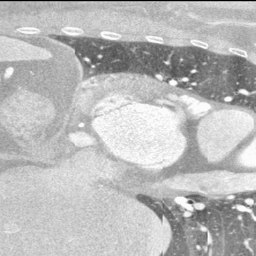
\includegraphics[width=0.18\textwidth]{image/chap04/seg/1_125input_ct.png}
    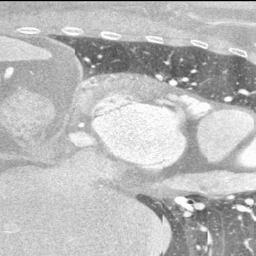
\includegraphics[width=0.18\textwidth]{image/chap04/seg/1_125lower.png}
    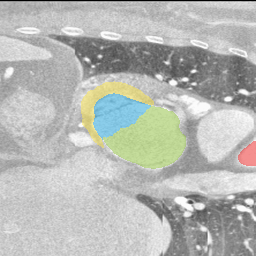
\includegraphics[width=0.18\textwidth]{image/chap04/seg/1_125pred.png}
    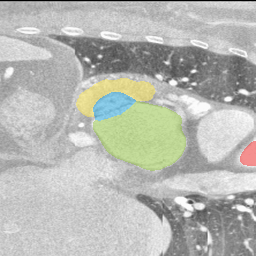
\includegraphics[width=0.18\textwidth]{image/chap04/seg/1_125upper.png}
    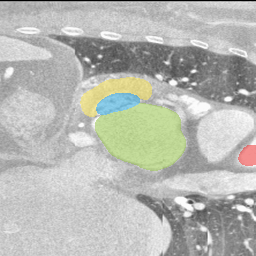
\includegraphics[width=0.18\textwidth]{image/chap04/seg/1_125gt.png}
    \\
    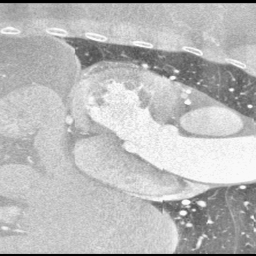
\includegraphics[width=0.18\textwidth]{image/chap04/seg/1_150input_ct.png}
    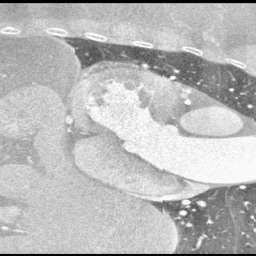
\includegraphics[width=0.18\textwidth]{image/chap04/seg/1_150lower.png}
    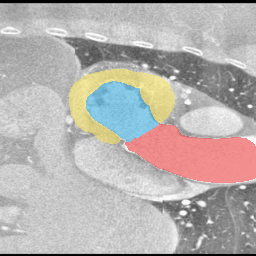
\includegraphics[width=0.18\textwidth]{image/chap04/seg/1_150pred.png}
    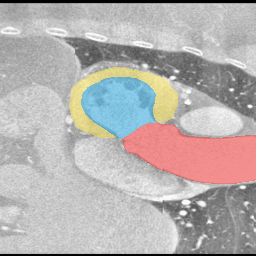
\includegraphics[width=0.18\textwidth]{image/chap04/seg/1_150upper.png}
    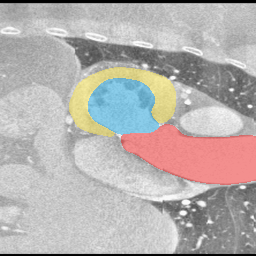
\includegraphics[width=0.18\textwidth]{image/chap04/seg/1_150gt.png}
    \\
    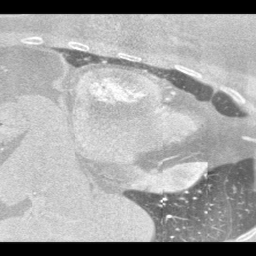
\includegraphics[width=0.18\textwidth]{image/chap04/seg/1_185input_ct.png}
    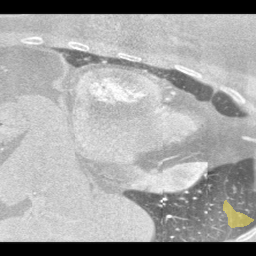
\includegraphics[width=0.18\textwidth]{image/chap04/seg/1_185lower.png}
    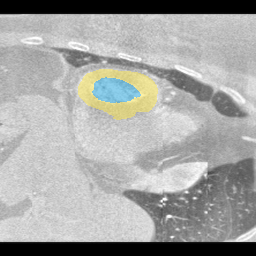
\includegraphics[width=0.18\textwidth]{image/chap04/seg/1_185pred.png}
    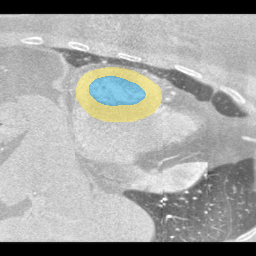
\includegraphics[width=0.18\textwidth]{image/chap04/seg/1_185upper.png}
    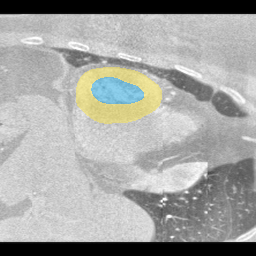
\includegraphics[width=0.18\textwidth]{image/chap04/seg/1_185gt.png}
    \\
    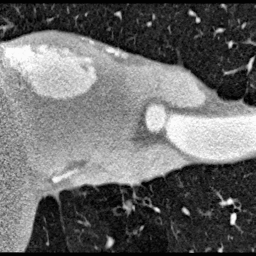
\includegraphics[width=0.18\textwidth]{image/chap04/seg/2_156input_ct.png}
    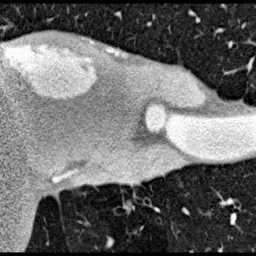
\includegraphics[width=0.18\textwidth]{image/chap04/seg/2_156lower.png}
    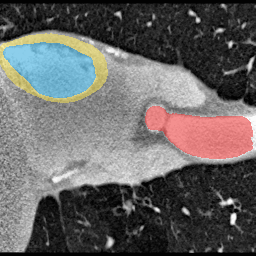
\includegraphics[width=0.18\textwidth]{image/chap04/seg/2_156pred.png}
    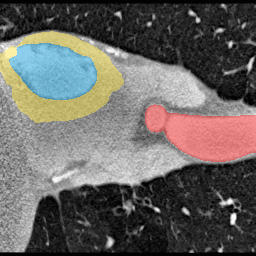
\includegraphics[width=0.18\textwidth]{image/chap04/seg/2_156upper.png}
    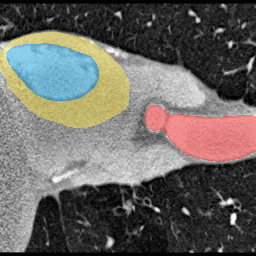
\includegraphics[width=0.18\textwidth]{image/chap04/seg/2_156gt.png}
    \\
    \makebox[0.18\textwidth]{\scriptsize CT image}
    \makebox[0.18\textwidth]{\scriptsize W/o adaptation}
    \makebox[0.18\textwidth]{\scriptsize Ours}
    \makebox[0.18\textwidth]{\scriptsize Supervised}
    \makebox[0.18\textwidth]{\scriptsize Ground Truth} 
    \caption{与相关方法的视觉分割效果比较}
    \label{fig:compare}
\end{figure}

视觉比较结果如图\ref{fig:compare}所示。可以看到,在不进行域自适应的情况下,网络很难对心脏结构进行有效的分割。而在进行域自适应之后,缓解了域位移问题带来的模型性能下降问题,分割器可以生成有解剖学意义的分割图,
\begin{figure}
    \centering
    \begin{subfigure}{\textwidth}
        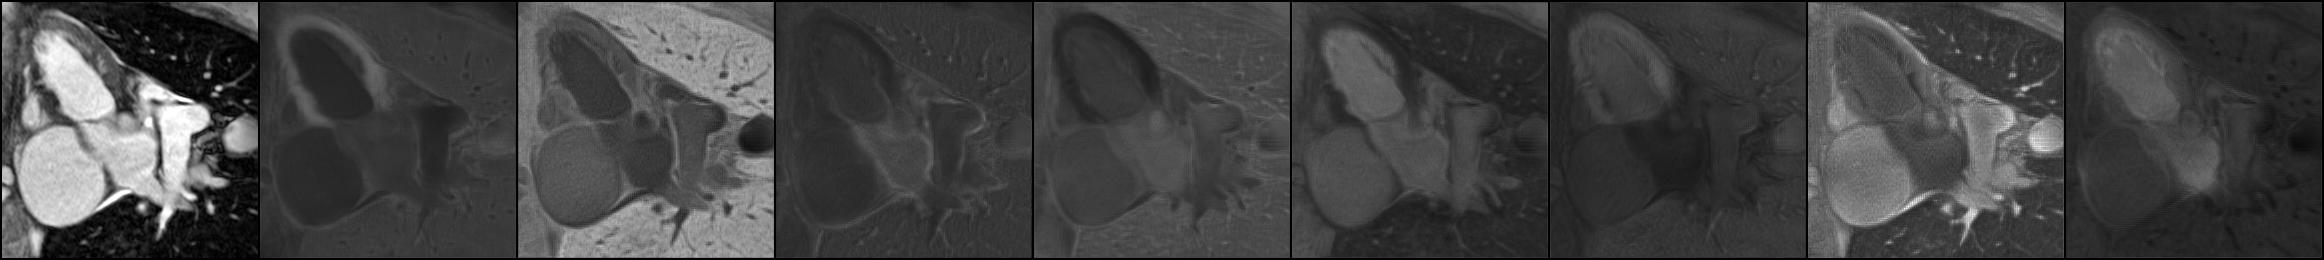
\includegraphics[width=1\textwidth]{image/chap04/attn_A.jpeg}
        \caption{$E_s^a$编码器对MRI图编码出的解剖学特征}
        \label{fig:attnA}
    \end{subfigure}
    \vfill
    \begin{subfigure}{\textwidth}
        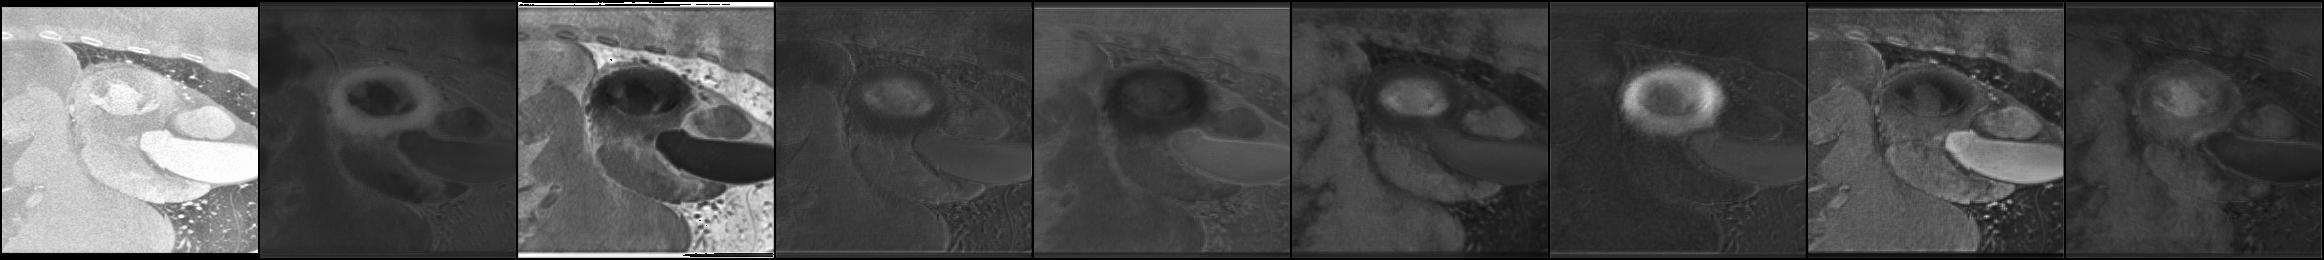
\includegraphics[width=1\textwidth]{image/chap04/attn_B.jpeg}
        \caption{$E_t^a$编码器对CT图编码出的解剖学特征}
        \label{fig:attnB}
    \end{subfigure}
    \caption{MRI图和CT图解剖学特征}
    \label{fig:attn}
    \end{figure}

\section{解耦表示}
如图\ref{fig:attn}所示,模型的解剖学特征编码器能够得到图像中有解剖学病理学意义的相关子结构,且在正交约束下,每个通道能提取到不同意义的病理区域,有效地促进了分割器的效果以及跨模态图像的生成。

\section{跨模态图像生成}
图\ref{fig:synthesis}中展示了跨模态图像的生成,从CT图转换到MRI图,可以看到,图像的外观转换为相应模态,同时保留了有效的语义区域用于分割,从中可以看出该框架有效地解耦模态特征和解剖学特征用于图像的生成。
\begin{figure}
    \centering
    \begin{subfigure}{\textwidth}
        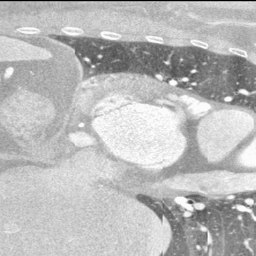
\includegraphics[width=0.18\textwidth]{image/chap04/seg/1_125input_ct.png}
        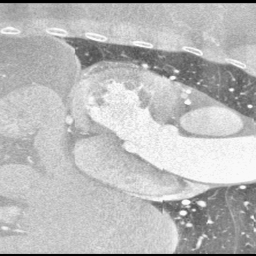
\includegraphics[width=0.18\textwidth]{image/chap04/seg/1_150input_ct.png}
        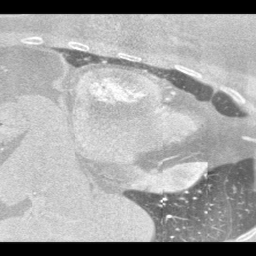
\includegraphics[width=0.18\textwidth]{image/chap04/seg/1_185input_ct.png}
        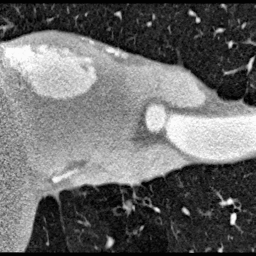
\includegraphics[width=0.18\textwidth]{image/chap04/seg/2_156input_ct.png}
        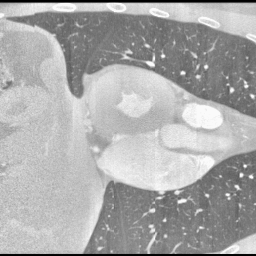
\includegraphics[width=0.18\textwidth]{image/chap04/seg/3_150input_ct.png}
        \caption{CT图}
        \label{fig:ct}
    \end{subfigure}
    \vfill
    \begin{subfigure}{\textwidth}
        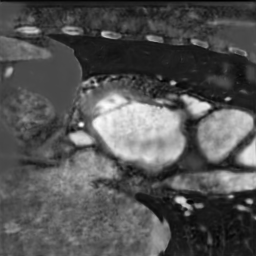
\includegraphics[width=0.18\textwidth]{image/chap04/seg/1_125fake_mr.png}
        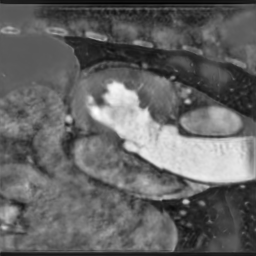
\includegraphics[width=0.18\textwidth]{image/chap04/seg/1_150fake_mr.png}
        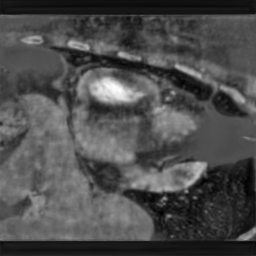
\includegraphics[width=0.18\textwidth]{image/chap04/seg/1_185fake_mr.png}
        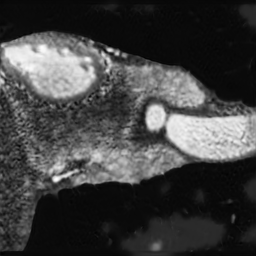
\includegraphics[width=0.18\textwidth]{image/chap04/seg/2_156fake_mr.png}
        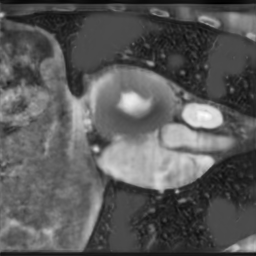
\includegraphics[width=0.18\textwidth]{image/chap04/seg/3_150fake_mr.png}
        \caption{生成的MRI图}
        \label{fig:fake_mri}
    \end{subfigure}
    \caption{跨模态图像生成:CT $\rightarrow$ MRI}
    \label{fig:synthesis}
    \end{figure}

